\documentclass{article}
\usepackage[LGR,T1]{fontenc}
\usepackage[utf8]{inputenc}
\usepackage[greek, english]{babel}
\usepackage{alphabeta}
\usepackage{natbib}
\usepackage{graphicx}
\usepackage{biblatex}
\addbibresource{references.bib}

\def\code#1{\texttt{#1}}

\usepackage{eso-pic}% http://ctan.org/pkg/eso-pic
\usepackage{lipsum}% http://ctan.org/pkg/lipsum

\title{Domain Model-v0.3}

\author{\\

\includegraphics[width=3in]{safeguard}\\[1ex]\\\\
}

\begin{document}

\maketitle

\newpage

Θεόδωρος Ντάκουρης - ntakouris@ceid.upatras.gr - 1054332: Editor \\
Βασίλειος Βασιλόπουλος - vvasil@ceid.upatras.gr - 1054410: Editor \\
Βάιος Λασκαρέλιας - laskarelias@ceid.upatras.gr - 1054432 Contributor, Reviewer \\
Νικόλαος Σουλτάνης - soultanis@ceid.upatras.gr - 1054319: Contributor, Reviewer \\

\begin{tabular}{|l|c|c|}
\hline
Όνοματεπώνυμο & email & Αριθμός μητρώου  \\
\hline
Θεόδωρος Ντάκουρης & ntakouris@ceid.upatras.gr & 1054332 \\
Βασίλειος Βασιλόπουλος & vvasil@ceid.upatras.gr &  1054410 \\
Νικόλαος Σουλτάνης & soultanis@ceid.upatras.gr & 1054319  \\
Βάιος Λασκαρέλιας & laskarelias@ceid.upatras.gr & 1054432 \\
Αντόν Παπά & papa@ceid.upatras.gr & 1054337 \\
\hline
\end{tabular}

\renewcommand{\contentsname}{Περιεχόμενα}
\tableofcontents

\section{Αλλαγές}
\subsection{v0.2}
Καθώς έγιναν προσθήκες, η ομάδα θα προχωρήσει σε συμπλήρωση attributes και functions στο επόμενο βήμα κατόπιν τα διαγράμματα sequence.

\begin{itemize}
    \item Προσθήκη RFID Card Data, RFID Reader Data, κατόπιν συγγραφής robustnes
    \item Παρομοίως, προσθήκη DocumentAttachment, AccessLevel
    \item Αφαιρέθηκαν PIN Entry Checks, Pin Entry 
    \item Αυτές οι προσθαφαιρέσεις διαπιστώθηκαν κατά τη δημιουργία Robustness
    \item Συμπληρώθηκαν μερικές συνδέσεις composition, γιατί στην προηγούμενη έκδοση υπήρχαν μόνο aggregations στη θέση τους.
    \hline
    \item Άρχισε η προσθήκη attributes σύμφωνα με τα διαγράμματα robustness.
    \item Η κλάση Access Log Data ενσωματώθηκε στο Access Log, καθώς ήταν πλεονασμός να υπάρχουν 2 διαφορετικές κλάσεις, οι οποίες είναι τόσο παρόμοιες.
\end{itemize}

\subsection{v0.3}
\begin{itemize}
    \item Αφαίρεση του Access Log Data και σύμπτυξή του με Access Logs λόγω πλεονασμού (συμπέρασμα με βάση τα sequence)
    \item Μετονομασία του RFID Scanner Data σε RFID Card Scanner Data λόγω naming inconsistency και επικάλυψη λειτουργικότητας
    \item Εισαγωγή στο domain model των Ui generated κλάσεων
    \item Εισαγωγή επίσης κάποιων κλάσεων που είναι boundary object αλλά δεν ανήκουν στο ui. Ανκήκουν σε μια ξεχωριστή κατηγορία 'hardware'. Αυτά είναι το RFID Card Scanner και το Sound Player.
    \item Αφαιρέθηκε η ιεραρχία check in-out access checks. Αναπαριστούνται καλύτερα σαν functions του RFID Card Scanner boundary object.
    \item Ενσωματώθηκαν τα UI στοιχεία στο Domain Model, συνδεδεμένα πλέον με τις υπόλοιπες κλάσεις.
    \item Αφαιρέθηκαν τα παιρετέρω classifiers καθώς θέλουμε το σύστημα να εντοπίζει οποιοδήποτε κίνδυνο ή γεγονός και όχι μόνο κάποια συγκεκριμένα.
    
\end{itemize}

\section{Λεκτικές Περιγραφές}

\subsection{Document Attachment}
Κάνει encapsulate λεπτομέρειες εγγράφου που γίνεται επισύναψη.

\subsection{Access Level}
Περιλαμβάνει επίπεδο προσβασιμότητας.

\subsection{RFID Card Data}
Περιέχει μερικά δεδομένα του employee καθώς και επίπεδο πρόσβασης, ημερομηνία έκδοσης-λήξης και άλλα.

\subsection{RFID Card Scanner Data}
Αντιπροσωπεύει δεδομένα που αποθηκεύονται σε κάθε 'unit' που σκανάρει κάρτες. Για παράδειγμα περιέχει τον sector, access level που βρίσκεται το unit.

\subsection{RFID Card Scanner}
Συνοψίζει τις βασικές λειτουργίες του third party card reader που θα χρησιμοποιήσουμε.Σκανάρει την κάρτα, ελέγχει την εγκυρότητα της καιι αν υπάρχει δικαίωμα πρόσβασης, επικοινωνώντας με τα κατάλληλα entities.

\subsection{Sound Player}
Ο μόνος του ρόλος είναι να παίξει τους βασικούς ήχους επιτυχίας-αποτυχίας.

\subsection{Human Entity}
Η βασική έννοια-μοντελοποίηση της ανθρώπινης παρουσίας στο project. Περιλαμβάνει βασικές πληροφορίες καθώς και δικαιώματα πρόσβασης.

\subsubsection{Guest}
Σηματοδοτεί το μικρότερο επίπεδο πρόσβασης, χωρίς να υπάρχουν πολλά στοιχεία στη βάση δεδομένων. Χρησιμοποιείται για έκδοση προσωρινής κάρτας πρόσβασης.

\subsubsection{Employee}
Συμβολίζει κάποιον υπάλληλο που θα έχει ημιμόνιμη παρουσία σοτ σύστημα με τακτικά check in και out, κατά την καθημερινή του εργασία.

\subsubsection{Security Guy}
Το κλασσικό προσωπικό ασφαλέιας, από τον φρουρό που κάθεται στην πόρτα μέχρι και τους ανώτερους επικεφαλείς. Ο καθένας έχει ένα PIN assigned και μπορεί να κάνει τις περισσότερες λειτουργίες στο σύστημα όπως να καταχωρήσει περιστατικό, να βγάλει κάρτα επισκέπτη ή κάρτα εργαζομένου.

\subsubsection{Chief Security Guy}
Ελάχιστοι υπάλληλοι προσωπικού είναι σε τέτοιο επίπεδο δικαιωμάτων. 

\subsection{Employee Shift}
Συμβολίζει την βάρδια κάθε εργαζομένου (ώρες, ημέρες). Μπορεί να χρησιμοποιηθεί και για τον έλεγχο πρόσβασης προσωρινής κάρτας guest.

\subsection{Employee Schedule}
Περιλαμβάνει το πρόγραμμα βαρδιών όλων των υπαλλήλων της εταιρίας. Θεωρούμε ότι προυπάρχει τέτοιο σύστημα διαχείρησης πόρων στην εταιρία και απλά κάνουμε integrate με αυτό.

\subsection{Notification Subsystem}
Συμβολίζει το 3rd party σύστημα ελέγχου της περιμέτρου από κάμερες και αισθητήρες.

\subsection{Drone}
Συνδέει το λογισμικό μας μαζί με κάποιο άλλο έτοιμο drone kit για enterprise χρήση που αναφέραμε και στο πλάνο του έργου (π.χ. skydio.com). Επικοινωνεί με το κομμάτι καταχώρησης περιστατικού ασφαλείας καθώς και κάποιες έξτρα λειτουργίες-εντολές όπως να πάει σε ένα σημείο, να γυρίσει στη βάση ή να κάνει image recognition.

\subsection{Incident Classifier}
Νευρωνικό δίκτυο το οποίο έχει εκπαιδευτεί κατάλληλα έτσι ώστε να μπορεί να αναγνωρίζει το είδος του περιστατικού μέσω φωτογραφίας.

\subsection{Central Office}
Το κύριο σύστημα επικοινωνίας μας με το προ-υπάρχων σύστημα της εταιρίας της οποίας πουλάμε το προϊόν μας. Στέλνει τα δεδομένα του κάθε περιστατικού.

\subsection{Incident Submission}
Το σύστημα που ο κάθε security guy μπορεί να αναφέρει περιστατικά. Προαιρετικά, εάν υπάρχει κάποιος συναγερμός ή ειδοποίηση από το σύστημα ασφαλείας περιμέτρου, ζητάει από τον αρμόδιο εκείνη τη στιγμή να καταχωρίσει περιστατικό αυτόματα.

\subsection{Access Log}
Ένα μικρό σύστημα στο οποίο δικαιώματα πρόσβασης έχει το προσωπικό ασφαλείας. Από εδώ γίνεται προβολή των τελευταίων περιστατικών καθώς και υπάρχουν φίλτρα αναζήτησης για τα περιστατικά που καταγράφινται εκεί.

\subsection{Security Incident}
Βασικές πληροφορίες περιστατικού ασφαλείας που καταχωρούνται.

\subsection{Popup Window}
Μια κλάση για τα βασίκα popup text windows

\subsection{MainMenu}
Το βασικό Menu της εφαρμογής, που φαίνονται και οι απαραίτητες ειδοποιήσεις απο τις υπόλοιπες λειτουργίες

\subsection{Ui\_InsertUserWidget}
Η οθόνη που εμφανίζεται κατα την προσθήκη καινούργιου χρήστη στο σύστημα

\subsection{Ui\_SendDroneWindow}
Η οθόνη που εμφανίζεται κατά την αποστολή των Drone σε κάποιο Sector.

\subsection{Ui\_SilentAlarmWindow}
Η οθόνη που εμφανίζεται εφόσον ο Security Guy ενεργοποιήσει τον συναγερμό.

\subsection{Ui\_PINEntryWidget}
Το widget που εμφανίζεται όταν το σύστημα ζητάει επιβεβαίωση pin

\subsection{Ui\_LivestreamWindow}
Η οθόνη που εμφανίζεται κατά την διάρκεια του Livestream όταν το Drone εντωπίσει κάποιο Incident, είναι μέσα στην Ui\_SendDroneWindow.

\subsection{Drone Control}
Περιέχει μεθόδους ελέγχου του Drone, και επικοινωνεί με το API του Drone που χρησιμοποιείται.

\subsection{Ui\_DeleteUserWidget}
To widget που εμφανίζεται για την διαγραφή κάποιου χρήστη.  



\section{Domain Model Diagram}
Για δική σας ευκολία παρακαλώ να δείτε πέρα από τα screenshots το παρακάτω view-only link από draw.io:

\url{https://drive.google.com/file/d/14eTfVLl6g93qm3I49ZbMsMJT_g3GaAAu/view?usp=sharing}

\newpage
\noindent\makebox[\textwidth]{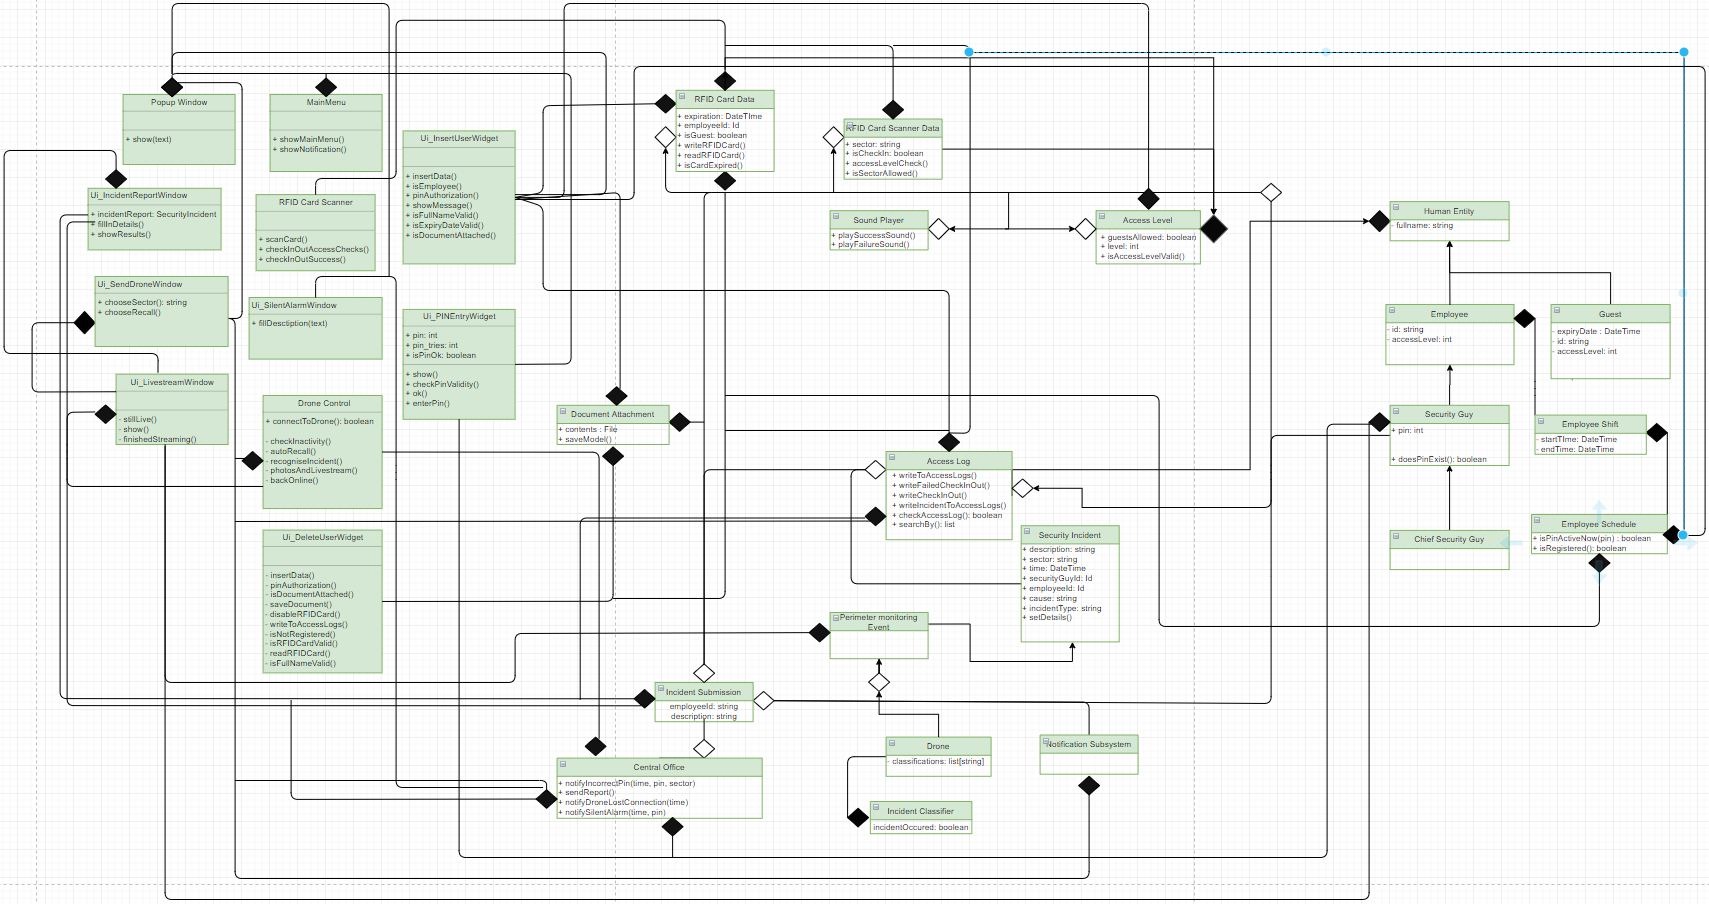
\includegraphics[width=\paperwidth]{domain-model.png}}\newpage

\newpage

\section{Εργαλεία}
Χρησιμοποιήθηκαν:
\begin{itemize}
    \item \LaTeX/Overleaf.com - Συγγραφή του παρόντος τεχνικού κειμένου
    \item Photoshop - Φωτογραφία Σελίδας Τίτλου
    \item draw.io - Σχεδιασμός διαγραμμάτων
\end{itemize}


\end{document}
